\section{Mixture Models}

In the previous chapter we have mentioned that it may happen that a likelihood function has multiple 
maxima and that sometimes it may be hard to impossible to find the global maximum (i.e. the maximum
with the overall highest likelihood value). Such a situation occurs whenever the probabilistic model
that we use to model our observations is a \textbf{mixture model}.

\begin{Definition}[Mixture Model]\label{def:mixtureModel}
Given any set of probability distributions $ P_{X1}, \ldots, P_{Xn} $ that are defined over the same
random variable $ X $ we define a mixture model as
$ P = \underset{i=1}{\overset{n}{\sum}} \alpha_{i}P_{Xi} $
where we require that $ \alpha_{i} \geq 0, 1 \leq i \leq n $ and 
$ \underset{i=1}{\overset{n}{\sum}} \alpha_{i} = 1 $.
We call the distributions $ P_{X1}, \ldots, P_{Xn} $ \textbf{mixture components} and their weights
$ \alpha_{i}, 1 \leq i \leq n $ \textbf{mixture weights}.
\end{Definition}

Mixture models are extremely useful whenever we have different ways to think about our data. Each way
of conceptualising our data can be encoded by one of the mixture components of the mixture model.
This can help us to build a better overall model of our data. Let us introduce a running example that
we will use for the rest of this section. 

\paragraph{Example of a mixture model} Assume we observe 10 sequences of coin tosses. Each sequence
contains 10 flips. We also know that there are 3 coins with which these sequences could possibly be
generated and for each sequence a different coin may have been used. Coin 1 is unbiased, coin 2 has
parameter $ \theta = 0.3 $ and coin 3 has parameter $ \theta = 0.65 $. 
 
We could use 
a multinomial distribution over coins to model our data. We would then employ maximum likelihood estimation 
and pick the coin that has the highest likelihood. However, this model might actually turn out to be
pretty bad because we are committing to picking only one coin, although we said in the beginning that
each sequence may possibly have been generated by a different coin. 

A mixture model comes to the rescue. Instead of assuming that only one coin has generated all 10 sequences,
we assume that all three coins have contributed to generating the 10 sequences. However, their distributions
may be unequal. This is exactly what the mixture weights capture. We will, as usual, call our data
$ x $. Also, each mixture component will be a binomial distribution, parametrized by the parameters of
the coins. This is enough to formulate our mixture model.
\begin{align}\label{eq:mixtureExample}
&P(X=x|\Theta_{1}^{3}=\theta_{1}^{3}, A = \alpha_{1}^{3}) 
= \alpha_{1}P(X=x|\Theta_{1}=0.4) \\
&+ \alpha_{2}P(X=x|\Theta_{2}=0.5) + \alpha_{3}P(X=x|\Theta_{3}=0.65) \nonumber
\end{align}

Notice that if we were given the mixture weights, estimating
the parameters of the mixture components would be easy: we would simply find the MLE for each mixture component. The mixture
model could then easily be constructed because the mixture weights are known. 

In the model given by Equation~\eqref{eq:mixtureExample} we are facing the opposite problem: we know the parameters of the
mixture components and we want to find good estimates for the mixture weights. How can we do this? Well, observe the constraints
on mixture weights in Definition~\ref{def:mixtureModel}. All mixture weights have to be non-negative and they have to sum to 1.
This means that we can interpret them as a probability distribution. In particular, this will be a distribution over parameters
of the mixture components (assuming that all mixture components have the same parametric form). That is, we get the following
equivalences:
\begin{equation}
\hskip 0.5cm \alpha_{1} = P(\Theta_{1} = \theta_{1}) \hskip 0.5cm \alpha_{2} = P(\Theta_{2} = \theta_{1}) \hskip 0.5cm \alpha_{3} = P(\Theta_{3} = \theta_{1})
\end{equation}
This means that we can rewrite our mixture model as
\begin{align} \label{eq:probabilisticMixtureModel}
&P(X=x) 
= P(\Theta_{1} = 0.4)P(X=x|\Theta_{1}=0.4) \\
&+ P(\Theta_{2} = 0.5)P(X=x|\Theta_{2}=0.5) + P(\Theta_{3} = 0.65)P(X=x|\Theta_{3}=0.65) \nonumber
\end{align}

Notice that in our examples we assume that we have only three possible binomial parameters, namely $ \theta_{1} = 0.4, \theta_{2} = 0.5, \theta_{3} = 0.65 $. 
Notice further that each summand
in \eqref{eq:probabilisticMixtureModel} is in fact a joint distribution by the chain rule so that we can again rewrite the model to
\begin{align}
P(X=x) &= P(X=x,\Theta_{1}=0.4) + P(X=x,\Theta_{2}=0.5) \\
&+ P(X=x,\Theta_{3}=0.65) \nonumber \\
&= \underset{i=1}{\overset{3}{{\sum}}} P(X=x,\Theta=\theta_{c_{i}}) \label{eq:marginal}
\end{align}
where line \eqref{eq:marginal} is a simple marginalisation step. Notice that we have just accomplished something impressive: we have given a probabilistic justification
for why mixture models do indeed model our data. Each mixture component-weight pair gives rise to a joint distribution over parameters and data but by summing over the 
possible parameters we get the probability of the data. By induction, we can easily show that mixture models are definable for any number of mixture components.

\begin{Exercise}
Show that a mixture model of size $ n $ is a model of the data, i.e. show that $  \alpha_{i}P_{i}(X=x) = P(X=x) $ if $ \alpha_{i} $ are mixture weights as 
defined in \ref{def:mixtureModel}.
\end{Exercise}

Notice that we have shown above that the formulation of mixture models as purely probabilistic model and as linear combinations of probability distributions are
equivalent. So why did we even bother to give a purely probabilistic justification? On the one hand, it is mathematically satisfying to trace back new concepts
to concepts that we are already familiar with (like joint distributions and the chain rule). More importantly, however, the probabilistic interpretation of mixture
weights allows us to estimate them using the maximum likelihood principle. This is something we could not have done, if we had regarded them solely as scale factors
for the mixture components. In our example there are only three possible parameters, meaning that we can impose a multinomial distribution over them. Let us
call the parameters of that multinomial $ \gamma_{1}, \gamma_{2}, \gamma_{3} $. Furthermore, remind yourself that our data consists of 100 i.i.d. Bernoulli
trial, $ k $ of which came up heads (with the usual restrictions on $ k $). Then our mixture model is

\begin{align}
P(X=x| \Gamma_{1}^{3}= \gamma_{1}^{3}) &\propto 0.4^{\gamma_{1}} \times (0.4^{k}0.6^{n-k}) \\
&+ 0.5^{\gamma_{2}} \times (0.5^{k}0.5^{n-k}) + 0.65^{\gamma_{3}} \times 0.65^{n}0.35^{n-k} \nonumber \\
&= 0.4^{\gamma_{1}+k}0.6^{n-k} + 0.5^{\gamma_{2}+k}0.5^{n-k} + 0.65^{\gamma_{3}+k}0.35^{n-k} \label{eq:multinomialLikelihood}
\end{align}

We have dropped the binomial and multinomial coefficients in the above equations, because they are constant and thus irrelevant to maximum likelihood estimation
of the multinomial parameters. This means that Equation~\eqref{eq:multinomialLikelihood} is proportional to our likelihood function and we will thus
maximize it. As usual, let us take the derivative of the log of that equation first. Since Equation~\eqref{eq:multinomialLikelihood} is a sum, we will maximize
each of the summands individually.

\begin{align}
\frac{d}{d\gamma_{1}} \log(0.4^{\gamma_{1}+k}0.6^{n-k}) &= \frac{d}{d\gamma_{1}} (\gamma_{1} + k)\times \log(0.4) + C = \frac{\gamma_{1} + k}{0.4} \\
\frac{d}{d\gamma_{2}} \log(0.5^{\gamma_{1}+k}0.5^{n-k}) &= \frac{d}{d\gamma_{2}} (\gamma_{2} + k)\times \log(0.5) + C = \frac{\gamma_{2} + k}{0.5} \\
\frac{d}{d\gamma_{3}} \log(0.65^{\gamma_{3}+k}0.35^{n-k}) &= \frac{d}{d\gamma_{3}} (\gamma_{3} + k)\times \log(0.65) + C = \frac{\gamma_{3} + k}{0.65}
\end{align}

If we set each of these derivatives to 0, we find that $ \gamma_{1} = 0.4 $, $ \gamma_{2} = 0.5 $ and $ \gamma_{3} = 0.65 $.

\section{Basics of Information Theory}

When we talk about \textit{information}, we often use the term in qualitative sense. We say things like \textit{This is valuable information} or 
\textit{We have a lack of information}. We can also make statements about some information being more helpful than other. For a long time, however,
people have been unable to quantify information. The person who succeeded in this endeavour was \href{https://en.wikipedia.org/wiki/Claude_Shannon}{Claude E. Shannon}
who with his famous 1948 article \textit{A Mathematical Theory of Communication} single-handedly created a new discipline: Information Theory! He also revolutionised
digital communication and can be seen as one of the main contributors to our modern communication systems like the telephone, the internet etc. 

The beauty about information theory is that it is based on probability theory and many results from probability theory seamlessly carry over to information theory.
In this chapter, we are going to discuss the bare basics of information theory. These basic will often be enough to understand many information theoretic arguments
that researchers make in fields like machine learning, psychology and linguistics.

Shannon's idea of information is as simple as it is compelling. Intuitively, if we are observing a realisation of a random variable, this realisation will surprise
if it is unlikely to occur according to the distribution of that random variable. However, if the probability for the realisation is very low, than on average it
will not occur very often, meaning that if we sample from the RV repeatedly, we will not be surprised very often. This will be the case when the probability
mass of the distribution is concentrated on only a small subset of its support. 

On the other hand, we will quite often be surprised,
if we cannot predict what the outcome of our next draw from the RV might be. This is exactly the case when the distribution over values of the RV is uniform. Thus,
we are going to be most surprised on average if we are observing realisations of a uniformly distributed RV.

Shannon's idea was that observing RVs that cause a lot of surprises is informative because we cannot predict the outcomes and with each new outcome we have effectively
learned something  (namely that the $ i^{th} $ outcome took on the value that it did). Observing RVs with very concentrated distributions is not very informative
under this conception because by just choosing the most probable outcome we can correctly predict most actually observed outcomes. Obviously, if I manage to predict
an outcome beforehand, it's occurrence is not teaching me anything.

The goal of Shannon was to find a function that captures this intuitive idea. He eventually found it and showed that it is the only function to have properties
that encompass the intuition. This function is called the \textbf{entropy} of a RV and it is simply the expected \textbf{surprisal} value.

\begin{Definition}[Surprisal]
The surprisal of an outcome $ x \in supp(X) $ of some RV $ X $ is
$$ -\log_{2}(P(X=x)) \ . $$
\end{Definition} 

\begin{Definition}[Entropy]
The entropy of a RV $ X $ is $ H(X) $ where $ H : X \rightarrow \mathbb{R}_{0+} $ is defined as
$$ H(X) := \mathbb{E}[-\log_{2}(P(X=x))] \ . $$
\end{Definition}

Figure~\ref{fig:binaryEntropy} shows the entropy of the Bernoulli distribution as a function of the
parameter $ \theta $. The entropy function of the Bernoulli is often called the \textbf{binary entropy}.
It measures the information of a binary decision, like a coin flip or an answer to a yes/no-question.
The entropy of the Bernoulli is 1 when the distribution is uniform, i.e. when both choices are equally 
probable. 

We also promised you at the outset of this section that you could easily transfer results from probability
theory.  So let us do this for a couple of cases. The most obvious connection seems to exist between
entropy and our results about expectations. For example, we know that expectation is linear, meaning
that
\begin{equation}
\mathbb{E}[aX + bY] = a\mathbb{E}[X] + b\mathbb{E}[Y]
\end{equation}
where $ X,Y $ are RVs that share the same set of values and $ a,b \in \mathbb{R} $ are constants.
\begin{figure}
\center
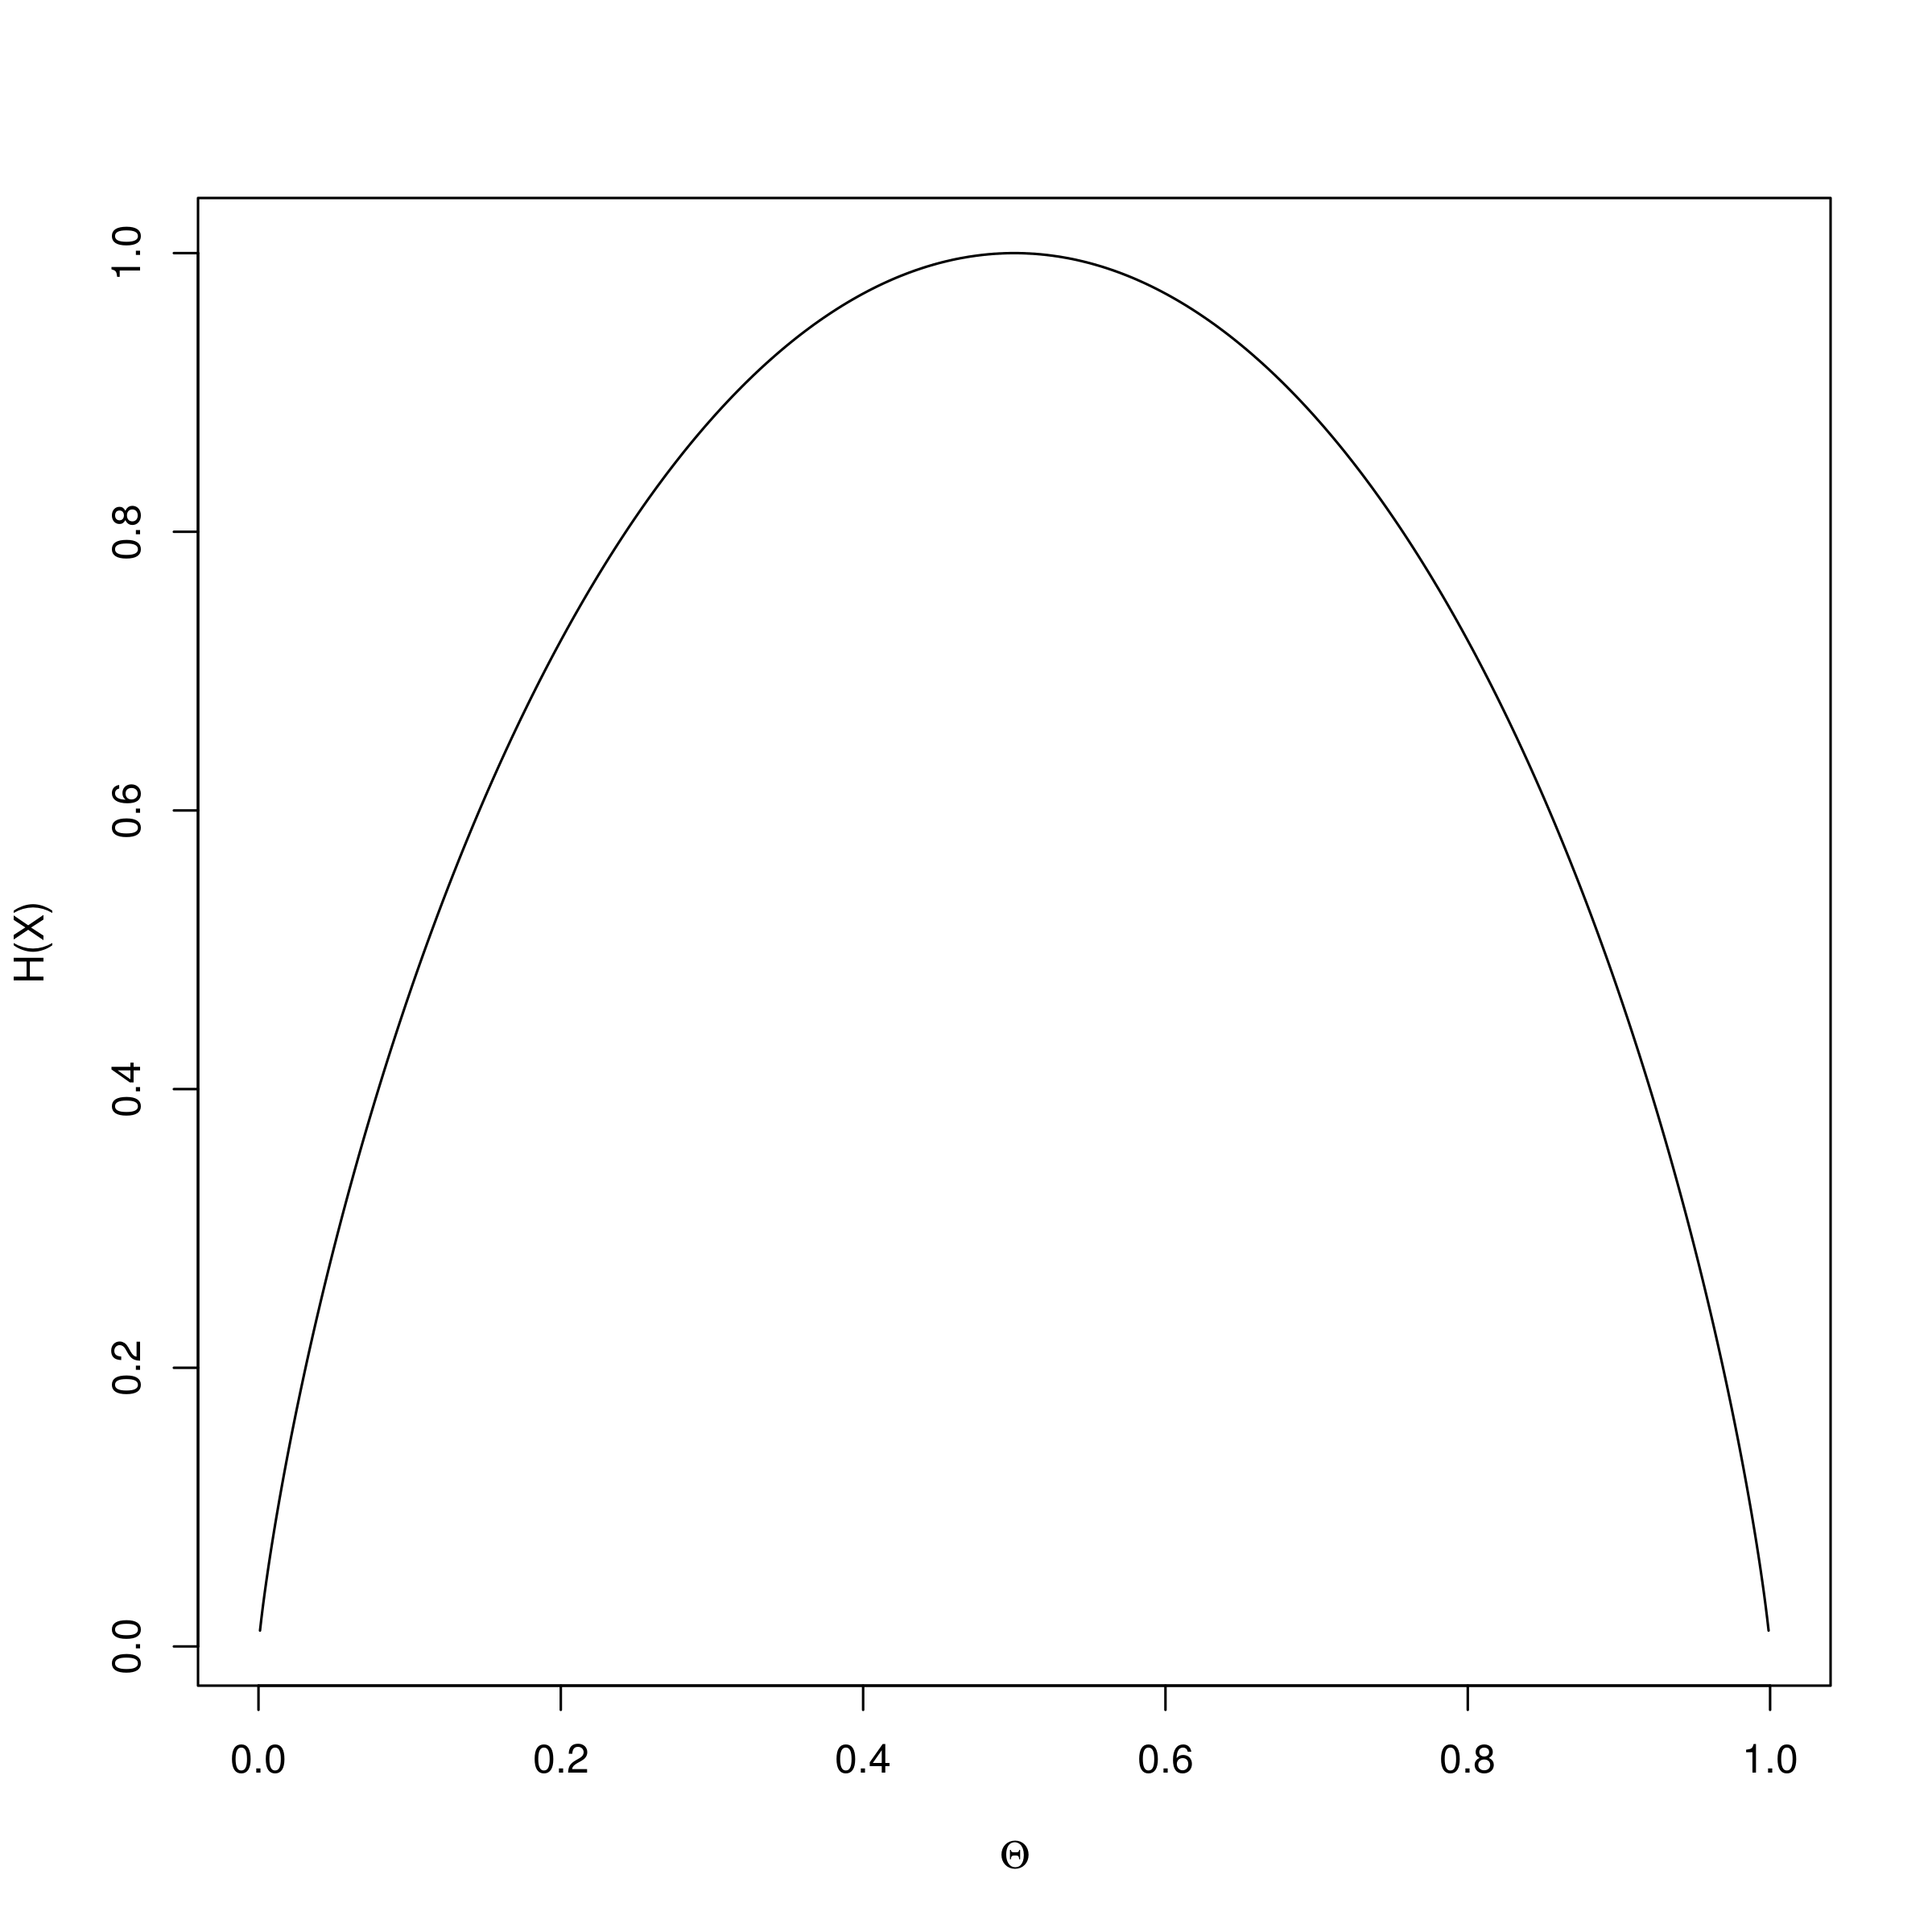
\includegraphics[scale=0.5]{binaryEntropy.png}
\caption{Binary entropy function.}
\label{fig:binaryEntropy}
\end{figure}

From the plot is it also easy to see that entropy is never negative. This is true for all entropy functions,
because they are just expectations of surprisal and surprisal is the negative logarithm of probabilities. 
Because $ \log(x) \leq 0 $ for $ x \in [0,1] $, it is clear that $ -\log(x) \geq 0 $ for $ x $ in the same
interval. Notice that from here on we will drop the subscript and by convention let $ \log = \log_{2} $.

A standard interpretation of the entropy is that it quantifies uncertainty. As we have pointed out
before, a uniform distribution means that you are most uncertain and indeed this is when the entropy
is highest. However, the more choices you have to pick from, the more uncertain you are going to be. 
The entropy function also captures this intuition. Notice that if a discrete distribution is uniform,
all probabilities are $ \frac{1}{|supp(X)|} $. Clearly, as we increase $ |supp(X)| $, we will decrease the
probabilities. By decreasing the probabilities, we increase their negative logarithms, and hence their
surprisal. Let us make this more formal.

\begin{Theorem}
A discrete RV $ X $ that follows uniform distribution and whose support has size $ n $ has entropy
$ H(X) = \log(n) $.
\end{Theorem}

\paragraph{Proof:}
\begin{align}
H(X) &= \underset{x \in supp(X)}{\sum}-\log(P(X=x))P(X=X) \\
&= \underset{x \in supp(X)}{\sum}\log(n)P(X=X) = \log(n)~~~~\square
\end{align}

\begin{Exercise}
You are trying to learn chess and you start by studying where chess grandmasters move their king when it
is positioned in the centre of the board. The king can move to any of the adjoining 8 fields. Since
you do not know a thing about chess yet, you assume that each move is equally probable. In this situation,
what is the entropy of moving the king?
\end{Exercise}

At the outset of this section we promised you that you could easily transfer results from probability 
theory to information theory. The most obvious connection exists between entropy and our results about
expectation. For example, we know that expectation is linear, meaning that for random variable $ X,Y $
that range over the same values and constants $ a,b \in \mathbb{R} $ it is true that
\begin{equation}
\mathbb{E}[aX+bY] = a\mathbb{E}[X] + b\mathbb{E}[Y] \ .
\end{equation}
Let us attempt the same thing for the entropy function.
\begin{equation}
H(aX + bY) = \underset{x \in supp(X)}{\sum} -\log(aX + bY)*P(X 
\end{equation}